\documentclass{sig-alternate}
\makeatletter
\def\@copyrightspace{\relax}
\makeatother

\begin{document}

% Copyright
\setcopyright{acmcopyright}

\title{
  % 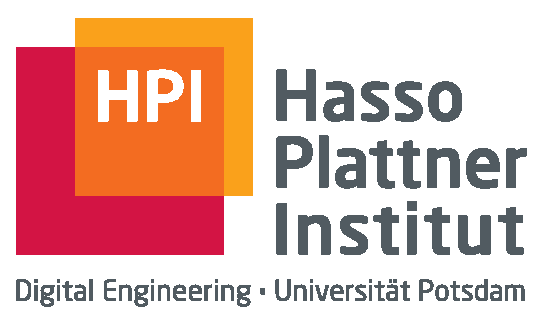
\includegraphics[width=0.2\textwidth]{hpi_logo_2017}\\
  \vspace{24pt}
  In-Memory Trajectory Analysis on Taxi Data
}
\subtitle{
  Seminar Trends and Concepts 3\\
  Summer Semester 2018
}

\numberofauthors{3}

\author{
  Marcel Jankrift\\
  Sebastian Kliem\\
  Toni Stachewicz\\[12pt]
  Supervisors:\\
  Dr. Matthias Uflacker, Keven Richly
}

\maketitle
\begin{abstract}
abstract
\end{abstract}


\keywords{test, test}

\section{Motivation}

\section{Data Sources}

\subsection{Data Cleansing}

\section{Application Prototype}

\subsection{System Architecture}

\subsection{Data Layouts}

\subsection{Optimizations}

\section{Benchmark Results}

\section{Future Work}

\section{Conclusion}

\section{References}
Generated by bibtex from your ~.bib file.  Run latex,
then bibtex, then latex twice (to resolve references)
to create the ~.bbl file.  Insert that ~.bbl file into
the .tex source file and comment out
the command \texttt{{\char'134}thebibliography}.

\end{document}
